\documentclass[tikz,border=0pt]{standalone}
\usepackage[utf8]{inputenc}
\usepackage[T1]{fontenc}
\usepackage{lmodern}
\usepackage{amsmath,amssymb}
\usetikzlibrary{arrows.meta,positioning,fit,calc,backgrounds,shapes.geometric,decorations.pathreplacing}
\definecolor{navy}{HTML}{163A5F}
\definecolor{blue}{HTML}{2C6EAF}
\definecolor{lightblue}{HTML}{EAF2F8}
\definecolor{midblue}{HTML}{CFE1F2}
\definecolor{graytext}{HTML}{4A5560}
\definecolor{lightgray}{HTML}{F4F6F8}
\definecolor{green}{HTML}{3C8D73}
\definecolor{lightgreen}{HTML}{E8F5EF}
\definecolor{red}{HTML}{B24A4A}
\definecolor{lightred}{HTML}{FBEDEE}
\tikzset{
  title/.style={font=\sffamily\bfseries\fontsize{18}{20}\selectfont,text=navy,anchor=west},
  subtitle/.style={font=\sffamily\bfseries\fontsize{11}{13}\selectfont,text=navy},
  body/.style={font=\sffamily\fontsize{9.2}{11}\selectfont,text=graytext,align=left},
  small/.style={font=\sffamily\fontsize{8}{9.4}\selectfont,text=graytext,align=left},
  tinylabel/.style={font=\sffamily\fontsize{7.2}{8.4}\selectfont,text=graytext},
  panel/.style={rounded corners=3pt,draw=midblue,fill=white,line width=0.6pt},
  box/.style={rounded corners=2pt,draw=midblue,fill=lightblue,line width=0.6pt},
  worker/.style={rounded corners=2pt,draw=blue,dashed,line width=0.7pt,fill=white},
  task/.style={rounded corners=2pt,draw=blue,fill=lightblue,minimum width=0.85cm,minimum height=0.55cm,font=\sffamily\bfseries\small,text=navy},
  file/.style={draw=blue,fill=white,minimum width=0.55cm,minimum height=0.42cm,font=\sffamily\small,text=navy},
  arr/.style={-{Stealth[length=2.4mm,width=1.8mm]},draw=blue,line width=0.9pt},
  arrthin/.style={-{Stealth[length=2mm,width=1.5mm]},draw=blue,line width=0.7pt},
  arrred/.style={-{Stealth[length=2mm,width=1.5mm]},draw=red,dashed,line width=0.8pt},
  arrgreen/.style={-{Stealth[length=2mm,width=1.5mm]},draw=green,dotted,line width=1pt}
}
\begin{document}

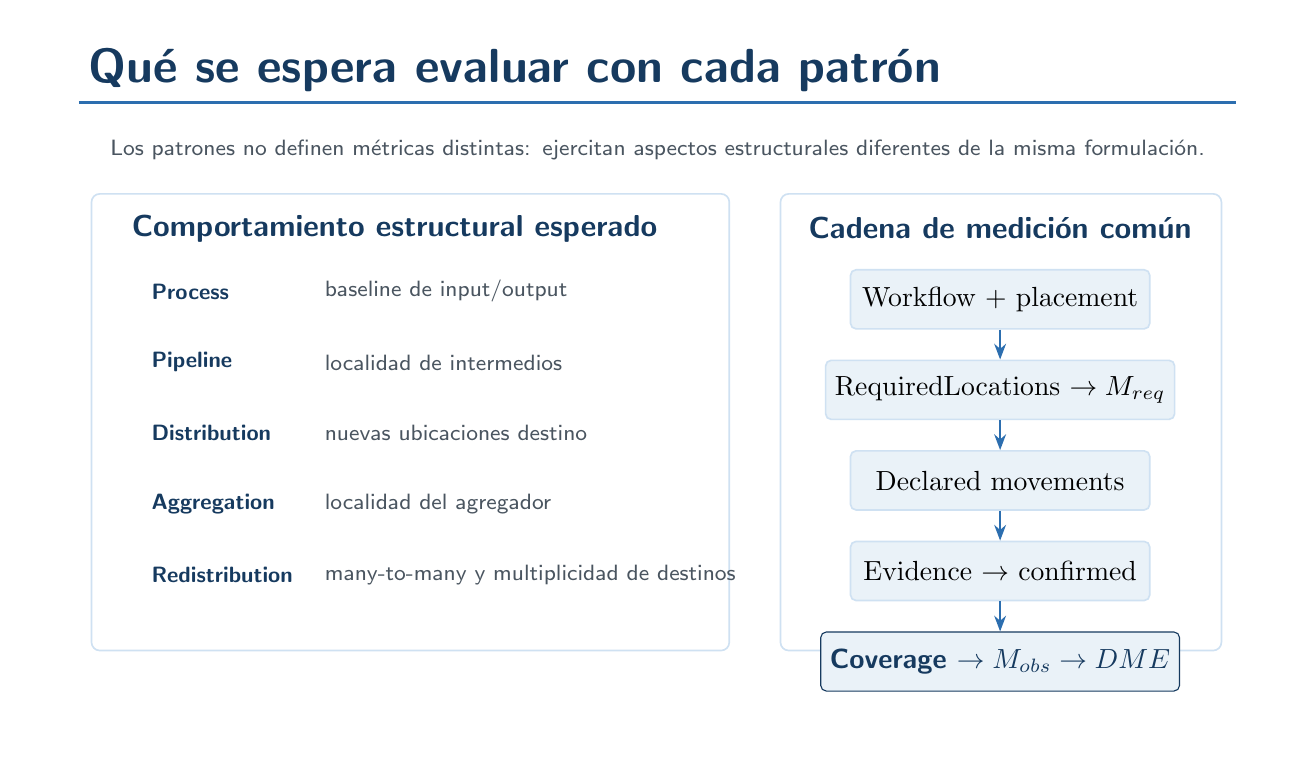
\begin{tikzpicture}[x=1cm,y=1cm]
\path[use as bounding box] (0,0) rectangle (16,9);
\node[title] at (0.65,8.45) {Qué se espera evaluar con cada patrón};
\draw[blue,line width=1pt] (0.65,8.05)--(15.35,8.05);
\node[small,text width=14.2cm,align=center] at (8,7.45) {Los patrones no definen métricas distintas: ejercitan aspectos estructurales diferentes de la misma formulación.};

\node[panel,minimum width=8.1cm,minimum height=5.8cm,anchor=north west] at (0.8,6.9) {};
\node[subtitle,anchor=west] at (1.2,6.45) {Comportamiento estructural esperado};
\foreach \y/\p/\t in {5.65/{Process}/{baseline de input/output},4.75/{Pipeline}/{localidad de intermedios},3.85/{Distribution}/{nuevas ubicaciones destino},2.95/{Aggregation}/{localidad del agregador},2.05/{Redistribution}/{many-to-many y multiplicidad de destinos}}{
\node[small,anchor=west,font=\sffamily\bfseries\fontsize{8}{9}\selectfont,text=navy] at (1.45,\y) {\p};
\node[small,anchor=west] at (3.65,\y) {\t};
}

\node[panel,minimum width=5.6cm,minimum height=5.8cm,anchor=north west] at (9.55,6.9) {};
\node[subtitle,align=center] at (12.35,6.45) {Cadena de medición común};
\node[box,minimum width=3.8cm,minimum height=0.75cm] (wp) at (12.35,5.55) {Workflow + placement};
\node[box,minimum width=3.8cm,minimum height=0.75cm] (rm) at (12.35,4.4) {RequiredLocations $\rightarrow M_{req}$};
\node[box,minimum width=3.8cm,minimum height=0.75cm] (dm) at (12.35,3.25) {Declared movements};
\node[box,minimum width=3.8cm,minimum height=0.75cm] (ev) at (12.35,2.1) {Evidence $\rightarrow$ confirmed};
\node[rounded corners=2pt,draw=navy,fill=lightblue,minimum width=3.8cm,minimum height=0.75cm,font=\sffamily\bfseries,text=navy] (met) at (12.35,0.95) {Coverage $\rightarrow M_{obs} \rightarrow DME$};
\draw[arrthin] (wp)--(rm); \draw[arrthin] (rm)--(dm); \draw[arrthin] (dm)--(ev); \draw[arrthin] (ev)--(met);
\end{tikzpicture}
\end{document}
